% !TEX root = ../main.tex

\section{Validation of the FW-H Method for Dipole Sources} \label{sec:dipole_validation}

With the FW-H numerical solver validated for monopoles, the validation is extended to dipole sources. As mentioned in Subchapter \ref{sec:dipole_derivation}, explicitly deriving the velocity terms for dipole sources is unviable, whcih led to the two approaches being tested separately to test the validity of each assumption and tests for cases on which these assumption are violated. The dual monopole approach will then redo all these cases to ensure its own validity. Table \ref{tab:dipole_validation_test_case} below summarises the test cases for the dipole; the column "Radius" refers to the permeable surface radius.

\begin{table}[H]
    \centering
    \caption{Summary of Dipole Validation Test Cases}
    \label{tab:dipole_validation_test_case}
    \begin{tabular}{p{1cm} p{4cm} p{1.8cm} p{1.8cm} p{1.8cm} p{2cm} p{1.5cm} l}
        \toprule
        \textbf{No} & \textbf{Assumption} & \textbf{Radius} & \textbf{$M_{source}$} & \textbf{$M_{observer}$} & \textbf{$x_{0,observer}$} & \textbf{Validity}\\
        \midrule
        1& Zero Relative Motion & $1.0m$ & [0,0,0] & [0,0,0] & [10,0,0] & Valid \\
        2& & $1.0m$ & [0.5,0,0] & [0.5,0,0] & [10,0,0] & Valid \\
        3& & $1.0m$ & [0.5,0,0] & [0,0,0] & [10,0,0] & Invalid \\

        4& Plane Wave & $500.0m$ & [0.5,0,0] & [0,0,0] & [500,0,0] & Valid \\
        5& & $1.0m$ & [0.5,0,0] & [0,0,0] & [1500,0,0] & Invalid \\
        
        6& Dual Monopole & $1.0m$ & [0,0,0] & [0,0,0] & [10,0,0] & - \\
        7& & $1.0m$ & [0.5,0,0] & [0.5,0,0] & [10,0,0] & - \\
        8& & $1.0m$ & [0.5,0,0] & [0,0,0] & [10,0,0] & - \\

        9& & $500.0m$ & [0.5,0,0] & [0,0,0] & [1500,0,0] & - \\
        10& & $1.0m$ & [0.5,0,0] & [0,0,0] & [1500,0,0] & - \\

        \bottomrule
    \end{tabular}
\end{table}

In the the following tests, only the Retarded Time algorithm will be used to allow the control surface to move along with the source. Only the finest discretisation resolution from the monopole tests will be used (275 grid points per wavelength and 30 time steps per period), to focus on validating the assumptions. Like the monopole cases, the source is set to radiate with the strength $Q(\tau)=sin(10\tau)$ and is initially placed at the origin.

\subsection{Dipole Derivation Validations} \label{subsec:dipole_derivation_validation}

Unlike the monopole validation, the co-translating test case is omitted for the dipole cases to isolate the  effects of a non-zero relative mach number. Therefore, the observer is stationary in all test cases. For all subsequent dipole test cases, the dipole axis and translation velocity are strictly imposed along the $x$-axis, while the observer maintains a transverse offset.

\begin{figure}[H]
    \centering
    \begin{subfigure}[b]{0.48\textwidth}
        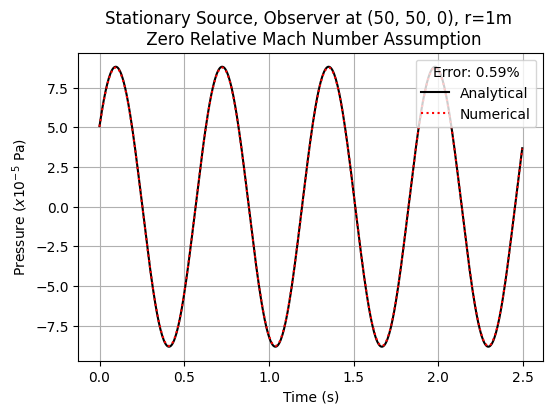
\includegraphics[width=\textwidth]{fig_dipole/dipole_near_valid.png}
        \caption{}
        \label{fig:near_valid}
    \end{subfigure}
    \hfill
    \begin{subfigure}[b]{0.48\textwidth}
        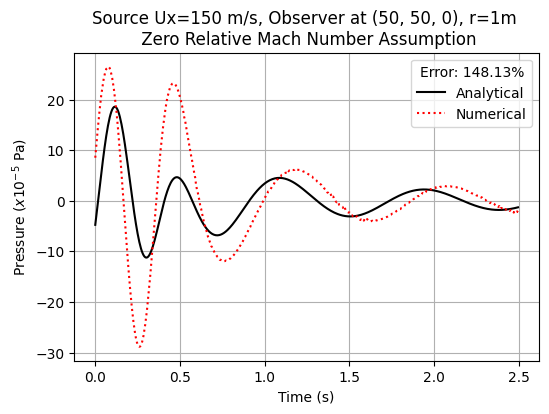
\includegraphics[width=\textwidth]{fig_dipole/dipole_near_invalid.png}
        \caption{}
        \label{fig:near_invalid}
    \end{subfigure}

    \vspace{0.5cm}
    
    \begin{subfigure}[b]{0.48\textwidth}
        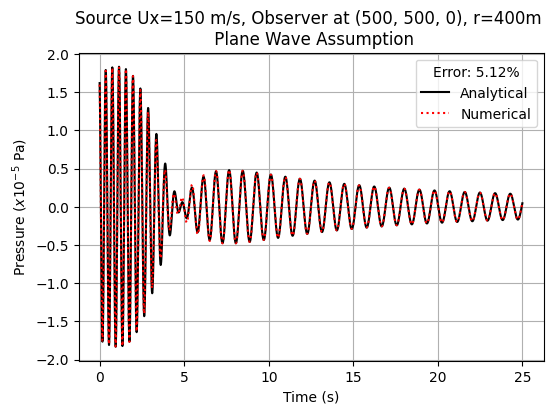
\includegraphics[width=\textwidth]{fig_dipole/dipole_far_valid.png}
        \caption{}
        \label{fig:far_valid}
    \end{subfigure}
    \hfill
    \begin{subfigure}[b]{0.48\textwidth}
        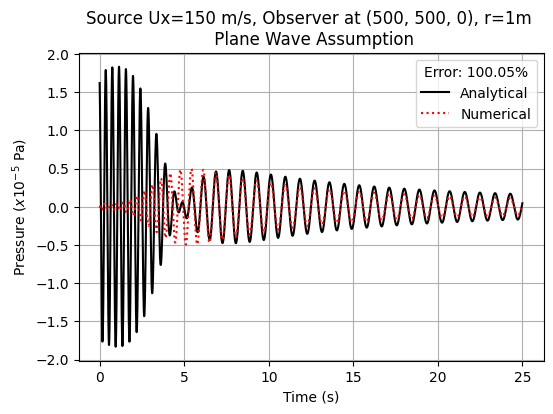
\includegraphics[width=\textwidth]{fig_dipole/dipole_far_invalid.png}
        \caption{}
        \label{fig:far_invalid}
    \end{subfigure}

    \caption[Comparison of analytical and numerical dipole.]{Comparison of analytical and numerical dipole.
    Top: zero relative Mach number case, with a) following, and b) violating the assumption.
    Bottom: plane wave case, with c) following, and d) violating the assumption.}
    \label{fig:dipole_validation}
\end{figure}

For the zero relative Mach number assumption, the tests examine how relative motion affect the results. In each case, the observer is put at $[50,50,0]$. To examine the integration accuracy, the first case examines a stationary problem, and the second one a relative motion problem, moving the source at $150m/s$ along the x-direction. In the plane wave assumption, the tests only examine the relative motion and putting the observer at $[500,500,0]$, to be in the "far-field." The control surface radius is expanded to $r=400m$ in the valid case and to $r=1m$ in the invalid case.

For stationary source and true far-field observer (Figures \ref{fig:near_valid} and \ref{fig:far_valid}), the results have good agreements at $<6\%$ error. However, introducing translation into the former and setting near-field surface to the latter violate the assumptions. For the $M_r=0$ case, the errors are due to the non-existent relative motion in Equation \ref{eq:dipole_u1}; for the plane wave assumption, the control surface being in the near-field of the source. The agreement as the source moves away from the observer is due to the observer eventually being in the physical far-field.

\subsection{Dual Monopole Validations} \label{subsubsec:dipole_dual_monopole_validation}
    
\begin{figure}[H]
    \centering
    \begin{subfigure}[b]{0.48\textwidth}
        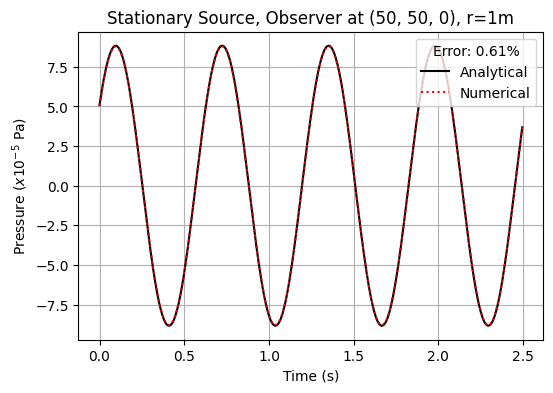
\includegraphics[width=\textwidth]{fig_dipole/dual_near_valid.png}
        \caption{}
        \label{fig:dual_near_valid}
    \end{subfigure}
    \hfill
    \begin{subfigure}[b]{0.48\textwidth}
        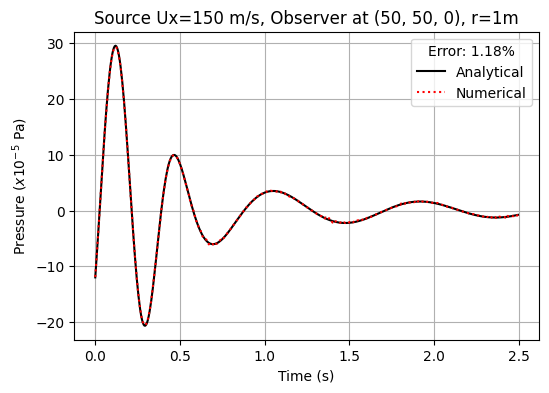
\includegraphics[width=\textwidth]{fig_dipole/dual_near_invalid.png}
        \caption{}
        \label{fig:dual_near_invalid}
    \end{subfigure}

    \vspace{0.5cm}
    
    \begin{subfigure}[b]{0.48\textwidth}
        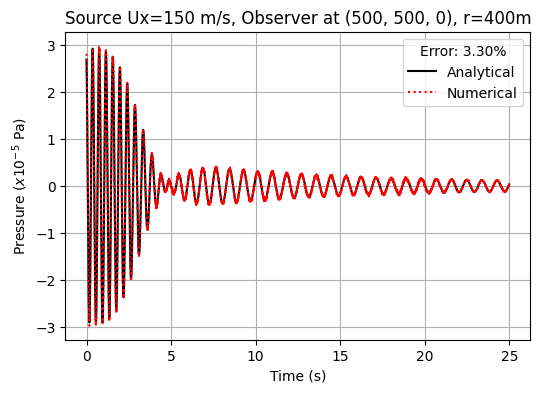
\includegraphics[width=\textwidth]{fig_dipole/dual_far_valid.png}
        \caption{}
        \label{fig:dual_far_valid}
    \end{subfigure}
    \hfill
    \begin{subfigure}[b]{0.48\textwidth}
        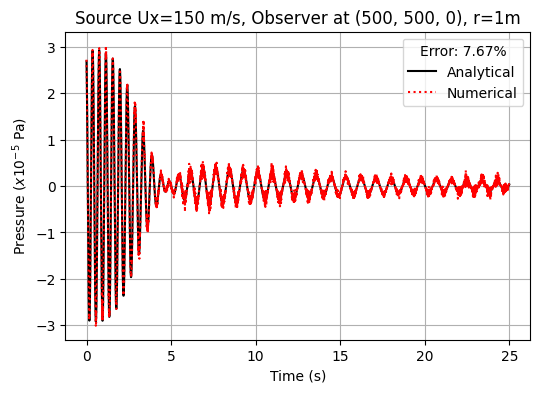
\includegraphics[width=\textwidth]{fig_dipole/dual_far_invalid.png}
        \caption{}
        \label{fig:dual_far_invalid}
    \end{subfigure}

    \caption[Comparison of analytical and numerical dipole validations using the dual monopole method.]{\centering Comparison of analytical and numerical dipole validations using the dual monopole method.
    Top: zero relative Mach number test cases, and bottom: plane wave test cases, the numerical results for all cases agree very well with the analytical solution.}
    \label{fig:dual_monopole_validation}
\end{figure}

In contrast to the analytical derivations, the dual-monopole method is significantly more robust in all cases, with highest error at $<8\%$. By superimposing two monopoles separated by $k\delta\ll1$, the solver retains the Doppler factor, which is omitted by the zero relative motion assumption. Similarly for the bottom figures, as the monopole was validated using a control surface in the near-field, the results generally agree in the cases which the far-field assumption failed when using the same control surface. It is noted that in Figure \ref{fig:dual_far_invalid}, the result exhibits more significant errors as the source moves away. This could be attributed to the limitations in the solver and will be discussed in the next chapter.

\subsection{Numerical Result Comparisons for Dipole Derivations and Dual Monopoles} \label{subsubsec:numerical_comparison}

\begin{figure}[H]
    \centering
    \begin{subfigure}[b]{0.48\textwidth}
        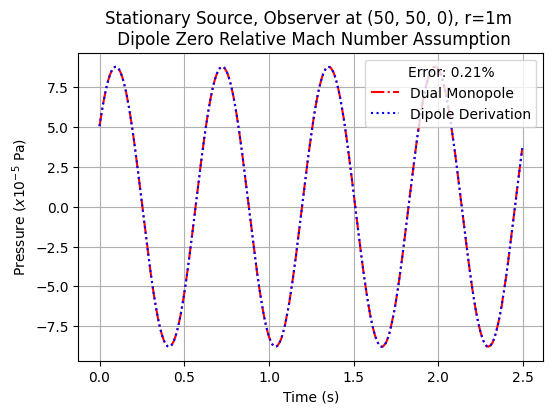
\includegraphics[width=\textwidth]{fig_dipole/dual_dipole_near_valid.png}
        \caption{}
        \label{fig:dual_dipole_near_valid}
    \end{subfigure}
    \hfill
    \begin{subfigure}[b]{0.48\textwidth}
        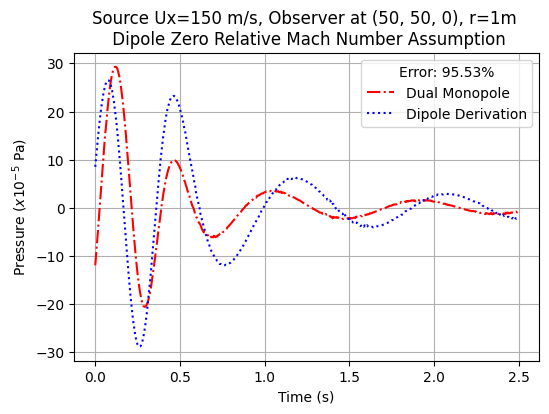
\includegraphics[width=\textwidth]{fig_dipole/dual_dipole_near_invalid.png}
        \caption{}
        \label{fig:dual_dipole_near_invalid}
    \end{subfigure}

    \vspace{0.5cm}
    
    \begin{subfigure}[b]{0.48\textwidth}
        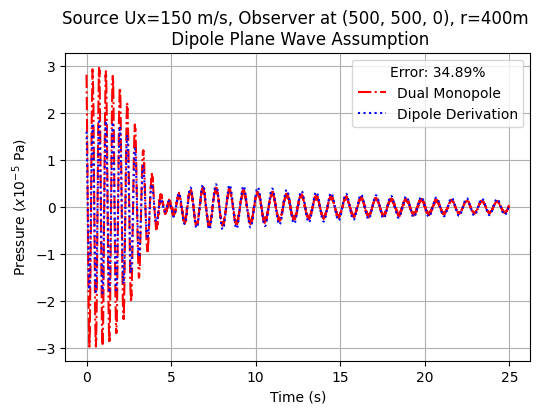
\includegraphics[width=\textwidth]{fig_dipole/dual_dipole_far_valid.png}
        \caption{}
        \label{fig:dual_dipole_far_valid}
    \end{subfigure}
    \hfill
    \begin{subfigure}[b]{0.48\textwidth}
        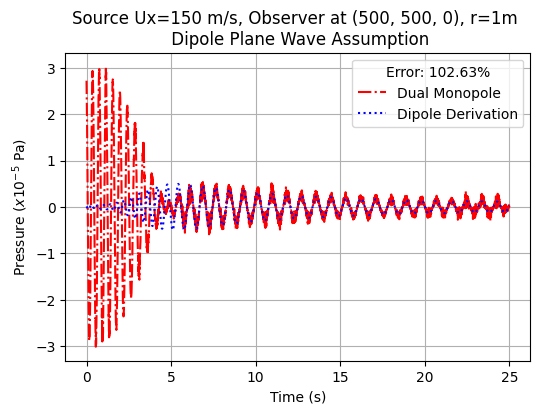
\includegraphics[width=\textwidth]{fig_dipole/dual_dipole_far_invalid.png}
        \caption{}
        \label{fig:dual_dipole_far_invalid}
    \end{subfigure}

    \caption[Comparison of numerical dipole validations.]{\centering Comparison of numerical dipole validations.
    Top: zero relative Mach number cases, and Bottom: plane wave cases. Left column are cases where the dipole assumptions followed the analytical solutions show good agreement with dual monopole. Right column shows where the dipole assumptions are violated.}
    \label{fig:dual_dipole_validation}
\end{figure}

Comparing the dipole derivations to the dual monopole approach shows that there are apparent deviations in results other than the stationary case. For Figure \ref{fig:dual_dipole_near_invalid}, it is obvious that the cause is the lack of Doppler effect in the assumption. Figure \ref{fig:dual_dipole_far_valid} is interesting due to a significant difference in amplitude as the sources approach the observers. Then as they move away, a good agreement in amplitude is observed. This is likely due to the imposing of the $x$-axis in the dipole source, because as it moves away, the $y$-axis contribution in the emission distance becomes insignificant.